\chapter{Application}
In this Chapter, the data is analyzed for cointegration relations. This will first be done pair wise by use of Engel Granger. Secondly it will be for all four simultaneously with the use of Johansen test. After the models are build, they will be used for forecasts, where the predictions will be measured against the validation data to test the precision of the models.


\section{Engel Granger Model Building}
To build the models, we first check for cointegration. This is done by making a linear model of all the $12$ possible combination of the cryptocurrencies. In theory cointegration is not directional, but in practice one acts as the regressand and therefore we check all $12$ combinations. Hereafter it is checked whether the model is $I(0)$ which is needed for it to be cointegrated, which is done be applying the \textit{adf.test} function in \textit{R}, which calculate the augmented Dickey Fuller test, to the residuals of the model. From this test, 4 models gave a p-value that reject the null hypothesis, meaning they are stationary, but to check if they are cointegrated one must check if their Critical value is larger than the given test statistic for the model. An example of this is shown for Solana \& Ethereum, here the acf, graph and histogram is made to check for constant and/or trend. This is because the Critical value changes if the data has a trend or a constant in what the augmented dickey fuller test deemed stationary.
\begin{figure}[h]
    \centering
    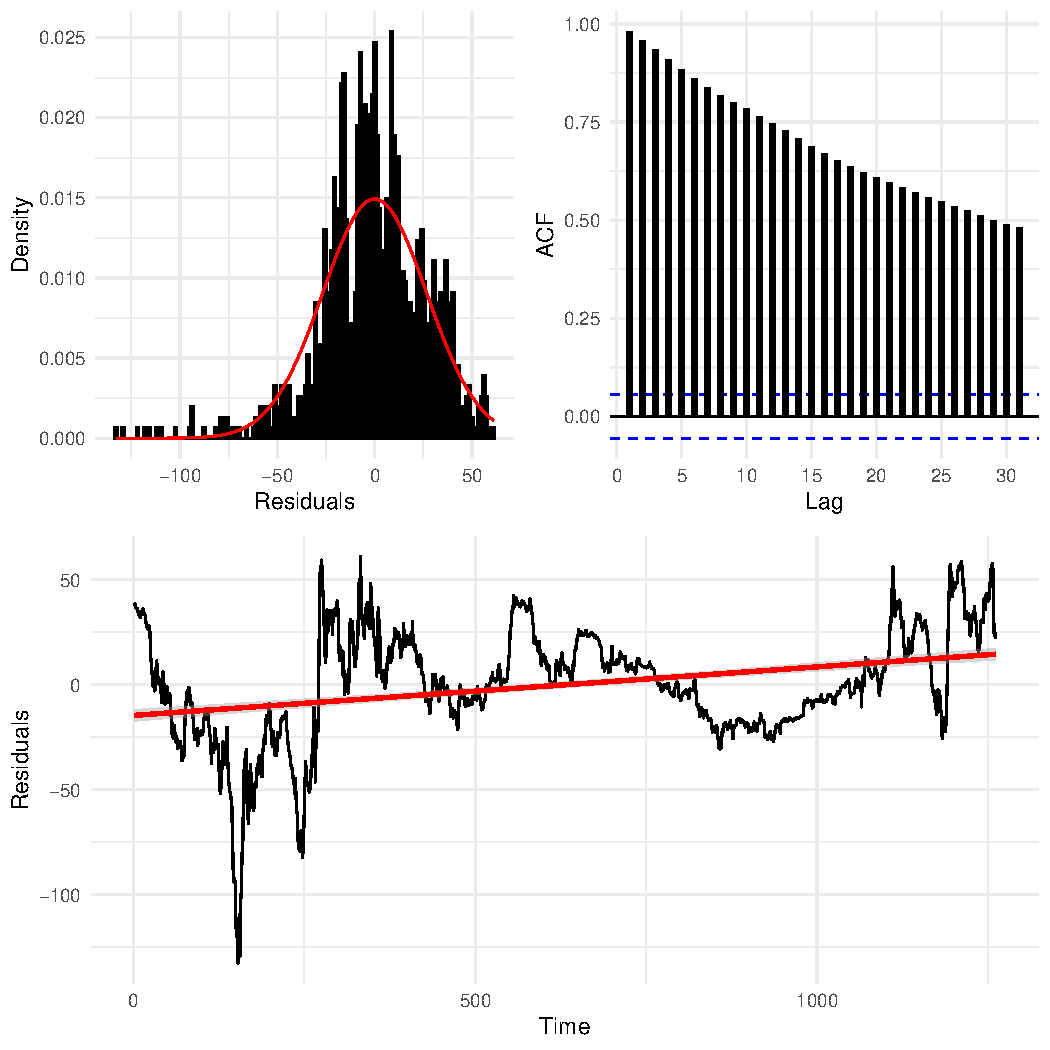
\includegraphics[width=0.4\linewidth]{1.Projekt_kode/Billeder/plot_grid_ADF_Solana-Ethereum.pdf}
    \caption{Caption}
    \label{fig:enter-label}
\end{figure}

\noindent From this figure it is clear from the ACF that a trend is present in the data, but no constant this give us a critical value with no constant but trend, as this could not be found the critical value with constant and trend is chosen. the given value is $-3.413$ (from IDK) the test-statistic for the given ADF test is $-4.059027$ and it can then be seen that $Critical\; Value>Test\;statistic$ the Null hypothesis can therefore be rejected and it is stationary. This is done for the other 3 models and they all reject the null hypothesis. This results in the following four pair wise currencies being $I(0)$ meaning they are cointegrating. 













\pause
\begin{center}
\begin{tabular}{cccc}
   Solana \& Ethereum \quad & \quad Ripple \& Ethereum\\\\
   Ethereum \& Solana \quad & \quad Ripple \& Solana
\end{tabular}
\end{center}
\pause
\noindent The four cases will be abbreviated, SOL\&ETH, XRP\&ETH, ETH\&SOL and XRP\&SOL respectively.(jp indsat) Next one VECM Model will be build using the above relations. This is because the cases where a cointegration relation was found, but only in one direction a VECM cannot be build. For those cases an ECM could be build instead. This will however not be done since we would have to forecast the predictor for the ECM using other means than cointegration. Therefore, the only model that will considered is the SOL\&ETH or ETH\&SOL since this will give us the same VECM model only with a difference in the position of ETH and SOL. To proceed with the analysis, we need to determine the optimal lag order for the model. First the function \textit{Varselect} is used to find the optimal lag order, the function evaluates it based on four criterions namely, Akaike Information Criterion, Hannan Quinn Criterion, Schwarz Criterion and Final prediction error. We have chosen to use AIC, since it theoretical is the best when predicting in the short term. The AIC scores for the SOL\&ETH have been plotted in Figure \ref{fig:AIC_plots}. The optimal lag order for a VAR model for SOL\&ETH, is found by visual interpretation of the plot in Figure \ref{fig:AIC_plots}.
\begin{figure}[H]
  \centering
  \subfloat[][Solana \& Ethereum]{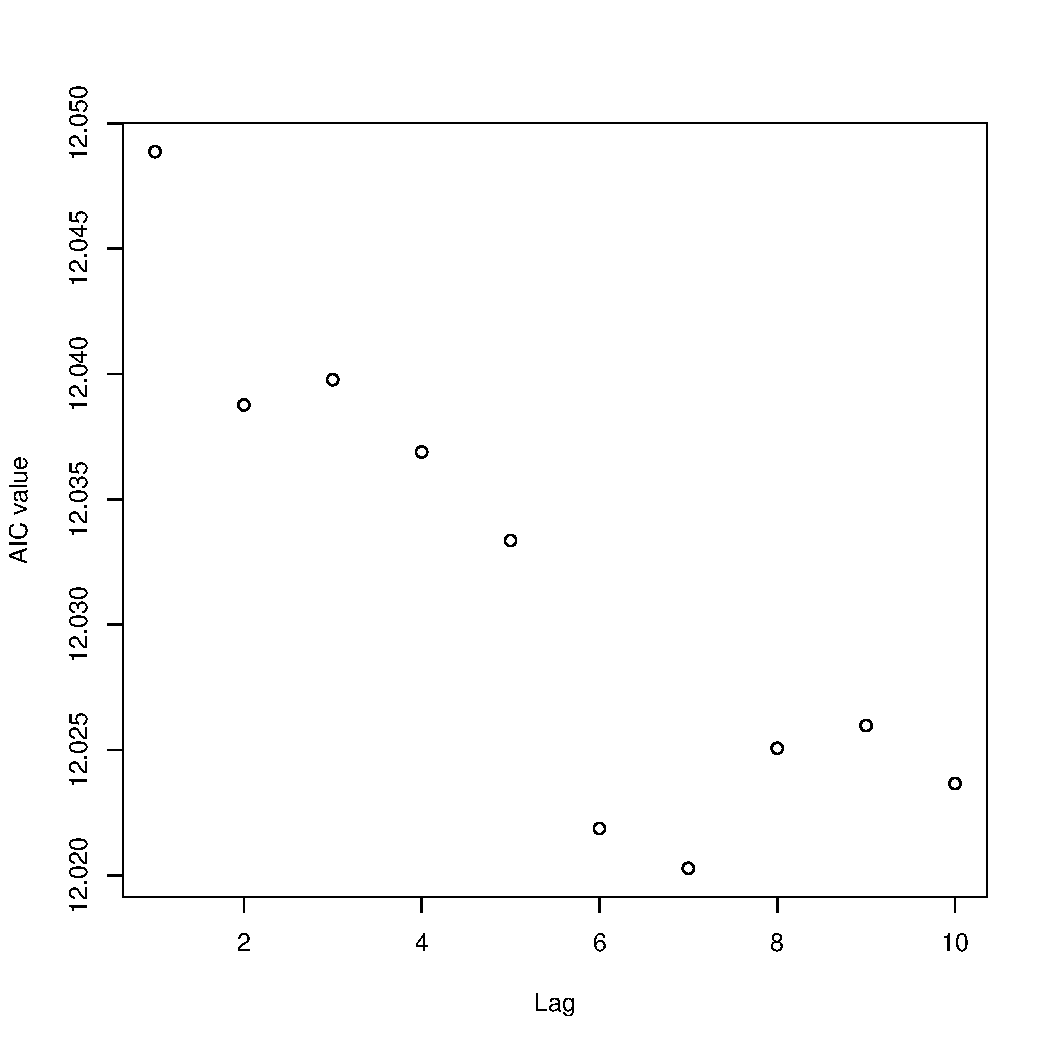
\includegraphics[width=.45\textwidth]{1.Projekt_kode/Billeder/AIC_Lag_for_SE.pdf}}\quad
  
  \caption{AIC values for SOL\&ETH}
  \label{fig:AIC_plots}
\end{figure}
\noindent The lag order is chosen to be $VAR(7)$. With the lag order determined. We can now build the VECM, where the lag order is simply one less than the $VAR$ counterpart.

\noindent The VECM is specified as follows, represented as a system of equations:\\

\begin{center}
    \textbf{SOL \& ETH}
\end{center}
$\text{Cointegrating Equation:} \quad  \beta = 1, \quad -0.03250492 \cdot \text{Ethereum} \\
\text{Equations:}$

\begin{align*}
\Delta \text{Solana}_t &= 
\underset{(0.0039)}{-0.0066} \cdot \text{ECT}_{t-1} + 
\underset{(0.1414)}{0.0657} + 
\underset{(0.0348)}{0.0413} \cdot \Delta \text{Solana}_{t-1} \\
&\quad + \underset{(0.0016)}{-0.0024} \cdot \Delta \text{Ethereum}_{t-1} + 
\underset{(0.0348)}{-0.0166} \cdot \Delta \text{Solana}_{t-2} \\
&\quad + \underset{(0.0016)}{0.0017} \cdot \Delta \text{Ethereum}_{t-2} + 
\underset{(0.0350)}{0.0403} \cdot \Delta \text{Solana}_{t-3} \\
&\quad + \underset{(0.0016)}{0.0019} \cdot \Delta \text{Ethereum}_{t-3} + 
\underset{(0.0349)^{**}}{0.0958} \cdot \Delta \text{Solana}_{t-4} \\
&\quad + \underset{(0.0017)}{-0.0005} \cdot \Delta \text{Ethereum}_{t-4} + 
\underset{(0.0351)^{**}}{-0.0941} \cdot \Delta \text{Solana}_{t-5} \\
&\quad + \underset{(0.0016)}{-0.0009} \cdot \Delta \text{Ethereum}_{t-5} + 
\underset{(0.0352)}{-0.0497} \cdot \Delta \text{Solana}_{t-6} \\
&\quad + \underset{(0.0016)^*}{0.0040} \cdot \Delta \text{Ethereum}_{t-6} + \epsilon_{\text{Solana},t}.
\end{align*}

\begin{align*}
\Delta \text{Ethereum}_t &= 
\underset{(0.0830)}{-0.0373} \cdot \text{ECT}_{t-1} + 
\underset{(3.0208)}{2.2306} + 
\underset{(0.7446)^*}{-1.5949} \cdot \Delta \text{Solana}_{t-1} \\
&\quad + \underset{(0.0349)}{-0.0267} \cdot \Delta \text{Ethereum}_{t-1} + 
\underset{(0.7433)^*}{-1.7485} \cdot \Delta \text{Solana}_{t-2} \\
&\quad + \underset{(0.0348)}{0.0573} \cdot \Delta \text{Ethereum}_{t-2} + 
\underset{(0.7471)}{-0.9073} \cdot \Delta \text{Solana}_{t-3} \\
&\quad + \underset{(0.0349)^*}{0.0800} \cdot \Delta \text{Ethereum}_{t-3} + 
\underset{(0.7467)^*}{1.8720} \cdot \Delta \text{Solana}_{t-4} \\
&\quad + \underset{(0.0353)}{-0.0123} \cdot \Delta \text{Ethereum}_{t-4} + 
\underset{(0.7490)}{0.4281} \cdot \Delta \text{Solana}_{t-5} \\
&\quad + \underset{(0.0352).}{-0.0668} \cdot \Delta \text{Ethereum}_{t-5} + 
\underset{(0.7512)}{-0.5645} \cdot \Delta \text{Solana}_{t-6} \\
&\quad + \underset{(0.0350)^*}{0.0886} \cdot \Delta \text{Ethereum}_{t-6} + \epsilon_{\text{Ethereum},t}.
\end{align*}

\begin{comment}
\begin{center}
   \textbf{ETH \& SOL}
\end{center}
$\text{Cointegrating Equation:} \quad  \beta = 1, \quad -25.22835 \cdot \text{Solana} \\
\text{Equations:} $
\begin{align*}
 \quad
\Delta \text{Ethereum}_t &= 
\underset{(0.0037)}{0.0011} \cdot \text{ECT}_{t-1} + 
\underset{(3.7672)}{1.9951} + 
\underset{(0.0348)}{-0.0304} \cdot \Delta \text{Ethereum}_{t-1} \\
&\quad + \underset{(0.7403)^*}{-1.6282} \cdot \Delta \text{Solana}_{t-1} + 
\underset{(0.0349)}{0.0570} \cdot \Delta \text{Ethereum}_{t-2} \\
&\quad + \underset{(0.7434)^*}{-1.6930} \cdot \Delta \text{Solana}_{t-2} + 
\underset{(0.0350)^*}{0.0835} \cdot \Delta \text{Ethereum}_{t-3} \\
&\quad + \underset{(0.7462)}{-0.8698} \cdot \Delta \text{Solana}_{t-3} + 
\underset{(0.0353)}{-0.0101} \cdot \Delta \text{Ethereum}_{t-4} \\
&\quad + \underset{(0.7478)^*}{1.8819} \cdot \Delta \text{Solana}_{t-4} + 
\underset{(0.0350)^*}{-0.0703} \cdot \Delta \text{Ethereum}_{t-5} \\
&\quad + \underset{(0.7480)}{0.4150} \cdot \Delta \text{Solana}_{t-5} + \epsilon_{\text{Ethereum},t}
\end{align*}
\begin{align*}
 \quad
\Delta \text{Solana}_t &= 
\underset{(0.0002)^*}{0.0004} \cdot \text{ECT}_{t-1} + 
\underset{(0.1761)}{-0.1083} + 
\underset{(0.0016).}{-0.0027} \cdot \Delta \text{Ethereum}_{t-1} \\
&\quad + \underset{(0.0346)}{0.0443} \cdot \Delta \text{Solana}_{t-1} + 
\underset{(0.0016)}{0.0016} \cdot \Delta \text{Ethereum}_{t-2} \\
&\quad + \underset{(0.0348)}{-0.0146} \cdot \Delta \text{Solana}_{t-2} + 
\underset{(0.0016)}{0.0020} \cdot \Delta \text{Ethereum}_{t-3} \\
&\quad + \underset{(0.0349)}{0.0411} \cdot \Delta \text{Solana}_{t-3} + 
\underset{(0.0017)}{-0.0004} \cdot \Delta \text{Ethereum}_{t-4} \\
&\quad + \underset{(0.0350)^{**}}{0.0969} \cdot \Delta \text{Solana}_{t-4} + 
\underset{(0.0016)}{-0.0010} \cdot \Delta \text{Ethereum}_{t-5} \\
&\quad + \underset{(0.0350)^{**}}{-0.0954} \cdot \Delta \text{Solana}_{t-5} + \epsilon_{\text{Solana},t}
\end{align*}
\end{comment}







\section{Johansen Model Building}
One of the advantages using the Johansen test, is its ability to detect cointegration among multiple time series at a time. This means that we are not only able to look at pairwise integrated series. We will throughout this secction both be using the trace test statistic explained in Section \cite{Johansen_test} and the Maximal Eigenvalue test. \\\\
The overall difference between the two tests is that the Trace test tests has $H_0$ saying there are at max $r$ cointegration relations versus $H_1$ stating the presence of more than $r$ cointegrating relations and has the statistic described in Section \cite{Johansen_test} \eqref{eq:lrmax_coint_r} where the Maximal Eigenvalue test has $H_0$ stating the presence of $r$ cointegrating relations whereas $H_1$ indicates the presence of $r+1$ cointegrating relations and has the test statistic $-Tln(1-\lambda_{r_0+1})$ meaning it tests each eigenvalue's influence individually.\\
Generally there is little to no difference between the results achieved through the two tests. The Trace test although are more likely to dismiss $H_0$ even though it might be true hence having higher probability of type 1 errors. At the same time the Trace test is more efficient in finding cointegration relations when they do exist and is more advantageous when multiple cointegration relations exists. Since both tests are beneficial in different scenarios it is preferable to perform both to see whether the comply with each other, and if not, examine further why this could be the case \citep{johansentestdifferences}.\\\\
After using the AIC then in the two day ahead prediction six lags gives the lowest AIC score meaning a $VAR(6)$ is the most efficient model whereas in the "ikke twodayahead" it is in the most instances preferable to use a $VAR(6)$-$VAR(7)$ model according to the AIC.


\subsection{Trace test}\label{subsec:johansen_trace}
Using Johansens trace test with a 5\% critical value is compared to the corresponding critical values for $r=0,\;r\leq1,\;r\leq 2,\;r\leq3$.
The results are computed using the R function $ca.jo$ and the results are plotted below.
\begin{table}[h!]
\centering
\begin{tabular}{|c|c|c|}
\hline
\textbf{Cointegrating Relations} & \textbf{Test Statistic} & \textbf{5\% Critical Values} \\ \hline
$r \leq 3$ & 0.32  & 8.18  \\ \hline
$r \leq 2$ & 13.85 & 17.95 \\ \hline
$r \leq 1$ & 42.19 & 31.52 \\ \hline
$r = 0$    & 83.51 & 48.28 \\ \hline
\end{tabular}
\caption{5\% $ca.jo$ results for the Johansen Trace test}
\label{tab:traceresults}
\end{table}
In Table \ref{tab:traceresults} it is seen that since the test statistic for $r=0$ and $r\leq1$ are more extreme than the critical values and thereby these null hypotheses are rejected  this indicates the presence of two cointegrating relations since this has a test statistic of 13.85 which is less than the corresponding critical value 17.95 and hence failing to reject the null hypothesis indicating the presence of two cointegrating relations.

\subsection{Maximum Eigenvalue test}
The Maximum Eigenvalue test is also used in order to see whether the two tests comply with each other. Once again th R function $ca.jo$ is used to compute the results and can be seen in the table below where the setup is the same as above.
\begin{table}[h!]
\centering
\begin{tabular}{|c|c|c|}
\hline
\textbf{Cointegrating Relations} & \textbf{Test Statistic} & \textbf{5\% Critical Values} \\ \hline
$r \leq 3$ & 0.32  & 8.18  \\ \hline
$r \leq 2$ & 13.53 & 14.90 \\ \hline
$r \leq 1$ & 28.33 & 21.07 \\ \hline
$r = 0$    & 41.32 & 27.14 \\ \hline
\end{tabular}
\caption{5\% $ca.jo$ results for the Johansen Maximun Eigenvalue test}
\label{tab:maximal_eigenvalue}
\end{table}
Just as concluded in Section \ref{subsec:classification_of_various_hypot} then the Maximum Eigenvalue test also indicates two cointegrating relations and there are therefore no issues regarding contradictions in the tests.

\subsection{Model Choice}
After both the Trace test and the Maximum Eigenvalue test suggests the presence of two cointegrating relations the next step is to apply the achieved conclusions in forecasting. The R function $ca.jo$ indicates that of the four eigenvalues only the two greatest, 0.0324140, 0.0223421, are significant enough to indicate a cointegrating relations.\\
Next the R function $cajorls$ is used to fit a VECM with two cointegrating relations. The error correction terms, hence the two $\beta$ vectors are given as seen in the table below:\\
\begin{table}[h!]
\centering
\begin{tabular}{|c|c|c|}
\hline
\textbf{Cryptocurrency} & $\b{\beta}_1$ & $\b{\beta}_2$ \\ \hline
Bitcoin $t-7$  & $1.000000$  & $0.0000$      \\ \hline
Ethereum $t-7$  & $-5.684342 \cdot 10^{-14}$ & $1.0000$    \\\hline
Solana $t-7$  & $-2.218088 \cdot 10^3$ & $-22.5305$    \\ \hline
Ripple $t-7$  & $1.248777 \cdot 10^6$  & $6121.3729$   \\ \hline
\end{tabular}
\caption{ECT coefficients for selected assets.}
\label{tab:ect_coefficients}
\end{table}

\noindent Next the VECM will be transformed into a VAR model, using the R function \textit{vec2var}, which will be used to forecast in the following section.



\section{Forecast}
To evaluate models ability to correctly forecast, we first look at a plot of a single 20-day-ahead prediction, where the prediction in blue are plotted against the true values in red and the $95\%$ confidence interval which is the shaded area. The black line is the actual values before forecasting. Secondly an 5-day-ahead forecast has been made iteratively, with each iteration adding another day to the training data set until the entire validation data set has been predicted upon. These predictions will be evaluated using the three different means mean absolute value (MAE), root mean square error(RMSE) and mean absolute percentage error(MAPE). The MAE is straight forward and measure the error value, while in the RMSE more weight is given to outliers. These two are a great combination, as a large difference between these two will indicate large outliers. The MAPE is used because it intuitively gives a great understanding of the errors. The formulas for calculation is given below:
\begin{align*}
    \text{MAE} = \frac{1}{n} \sum_{i=1}^{n} |y_i - \hat{y}_i|, \quad \text{RMSE} = \sqrt{\frac{1}{n} \sum_{i=1}^{n} (y_i - \hat{y}_i)^2}, \quad \text{MAPE} = \frac{1}{n} \sum_{i=1}^{n} \left| \frac{y_i - \hat{y}_i}{y_i} \right|\cdot 100.
\end{align*}
\noindent Where $y_i$ is the actual value and $\hat{y}_i$ is the predicted value and is the number of observation.

\subsection{Engel Granger}
First the 20-day-ahead predictions plot will be looked at. These are however not very representable of the actual accuracy of the models, since it is just a single prediction. It does however give an insight into whether the model is able to capture the movements of the actual data.\\
\begin{center}
    \textbf{SOL \& ETH}
\end{center}
\begin{figure}[H]
  \centering
  \subfloat[][Solana]{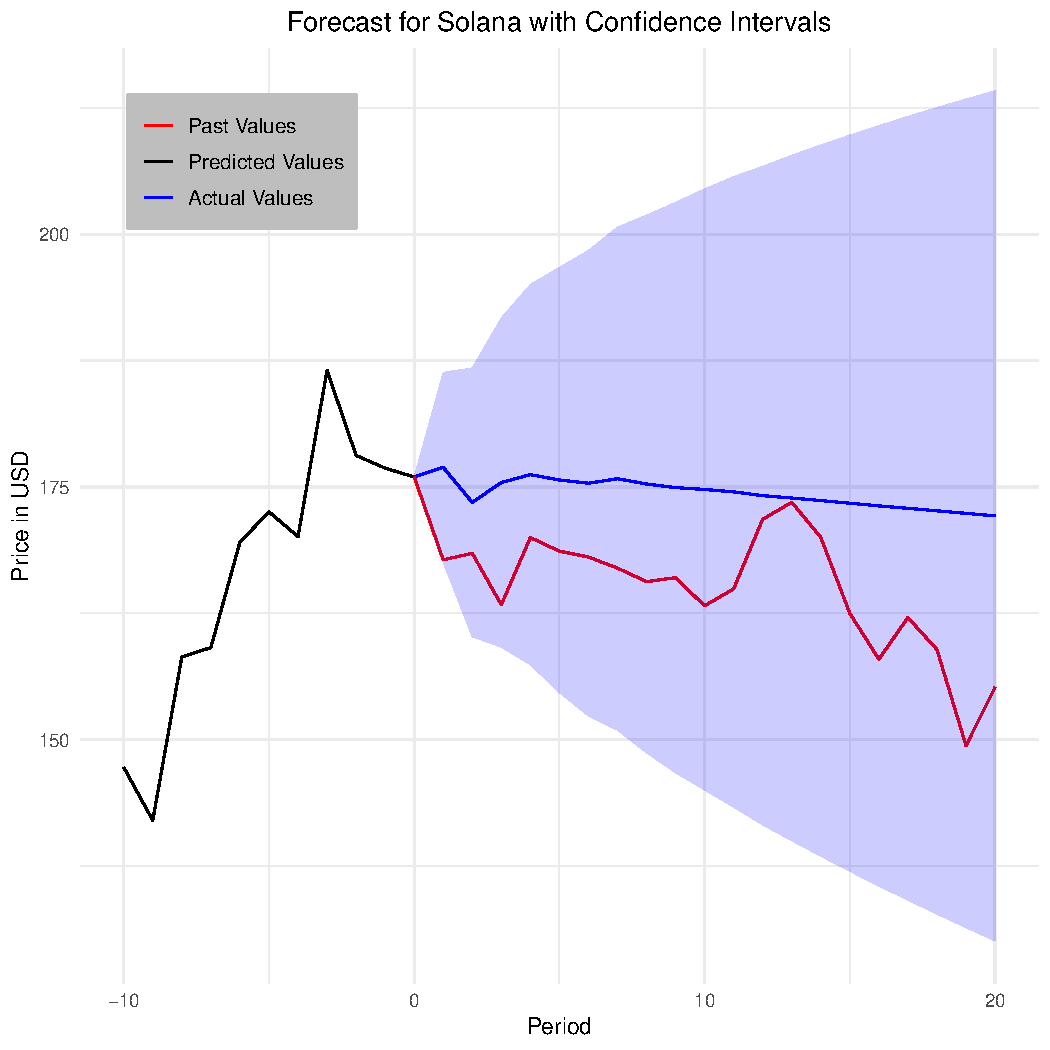
\includegraphics[width=.45\textwidth]{1.Projekt_kode/Billeder/20_day_ahed_Solana_from_Solana_Ethereum.pdf}}\quad
  \subfloat[][Ethereum]{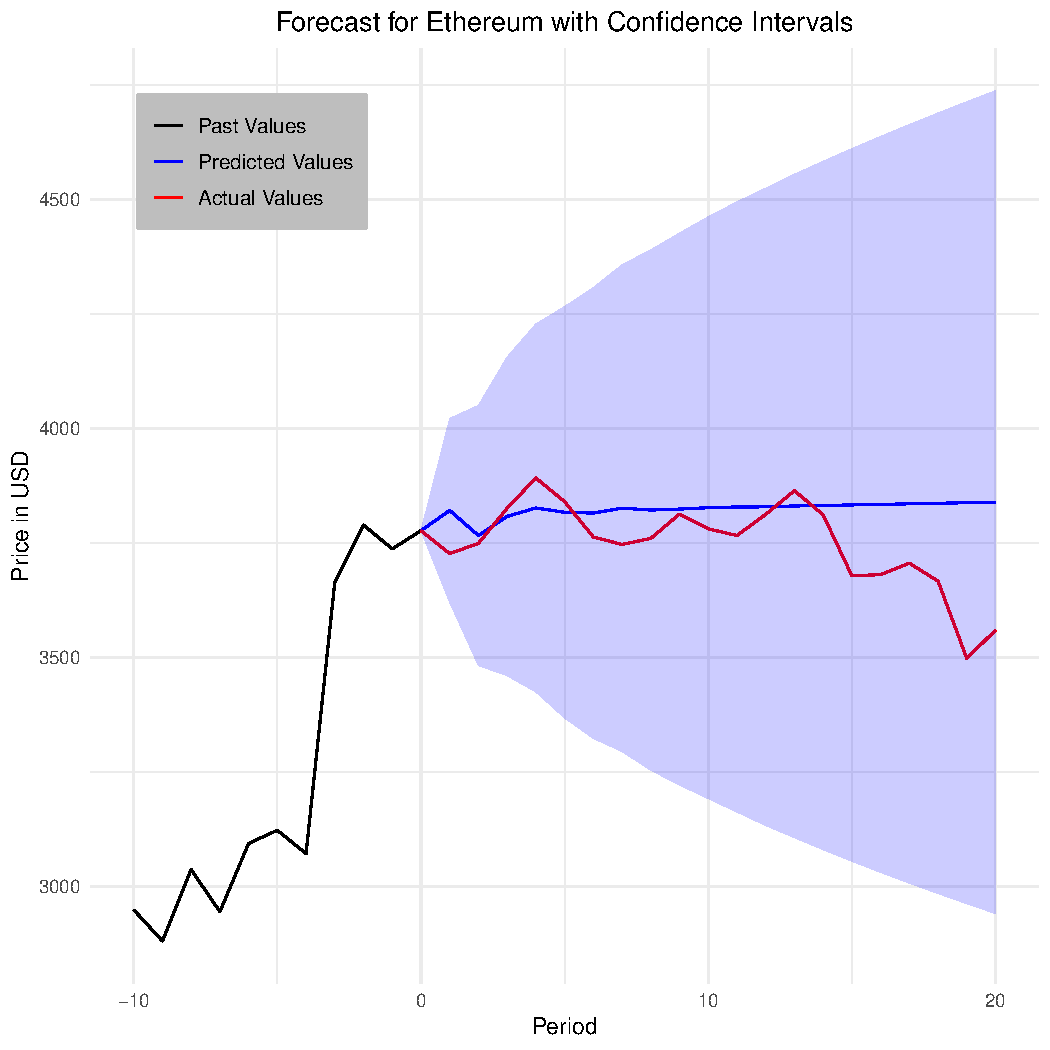
\includegraphics[width=.45\textwidth]{1.Projekt_kode/Billeder/20_day_ahed_Ethereum_from_Solana_Ethereum.pdf}}
  \caption{20-day-ahead prediction plot}
  \label{fig:SOL_ETH_20_DAY_plot}
\end{figure}
\begin{comment}
\begin{center}
    \textbf{ETH \& SOL}
\end{center}

\begin{figure}[H]
  \centering
  \subfloat[][Ethereum]{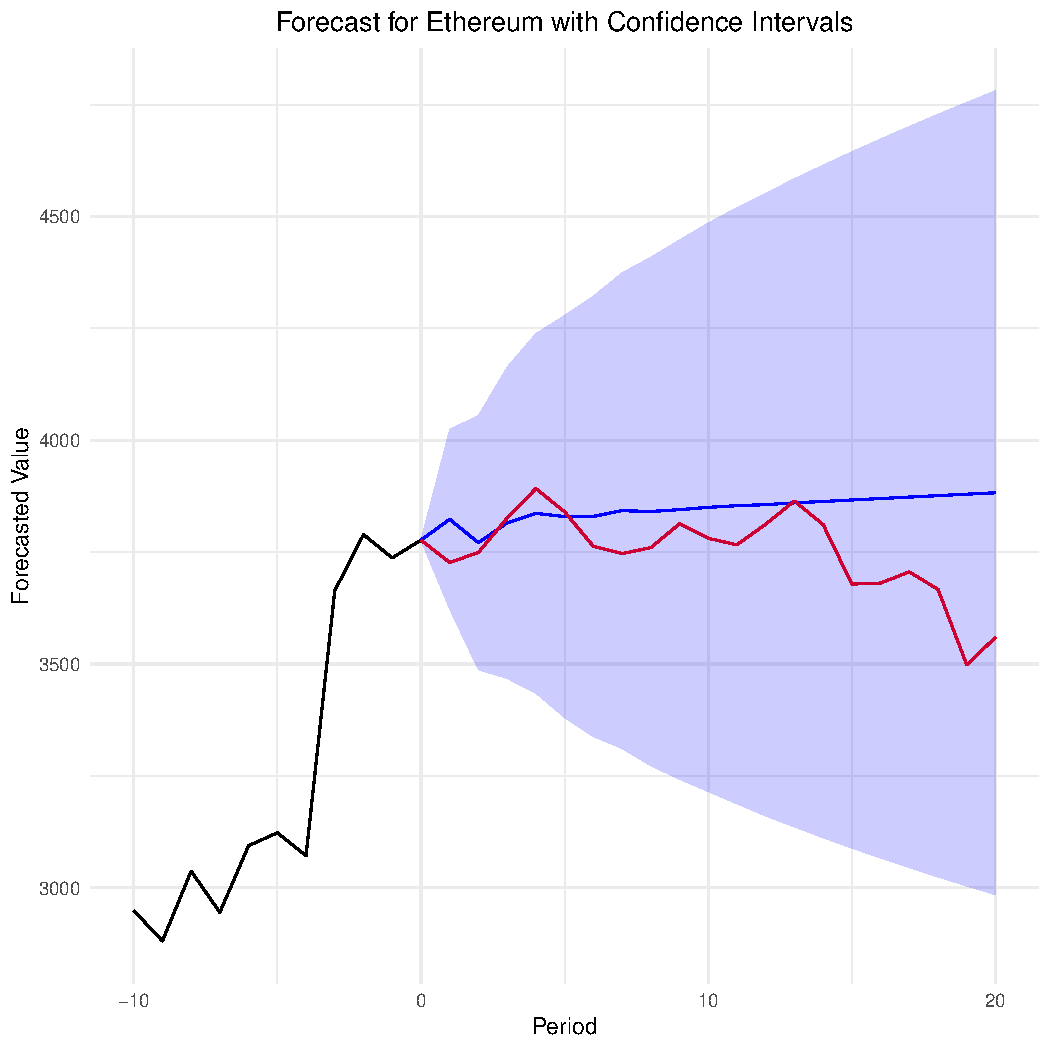
\includegraphics[width=.45\textwidth]{1.Projekt_kode/Billeder/20_day_ahed_Ethereum_from_Ethereum_Solana.pdf}}\quad
  \subfloat[][Solana]{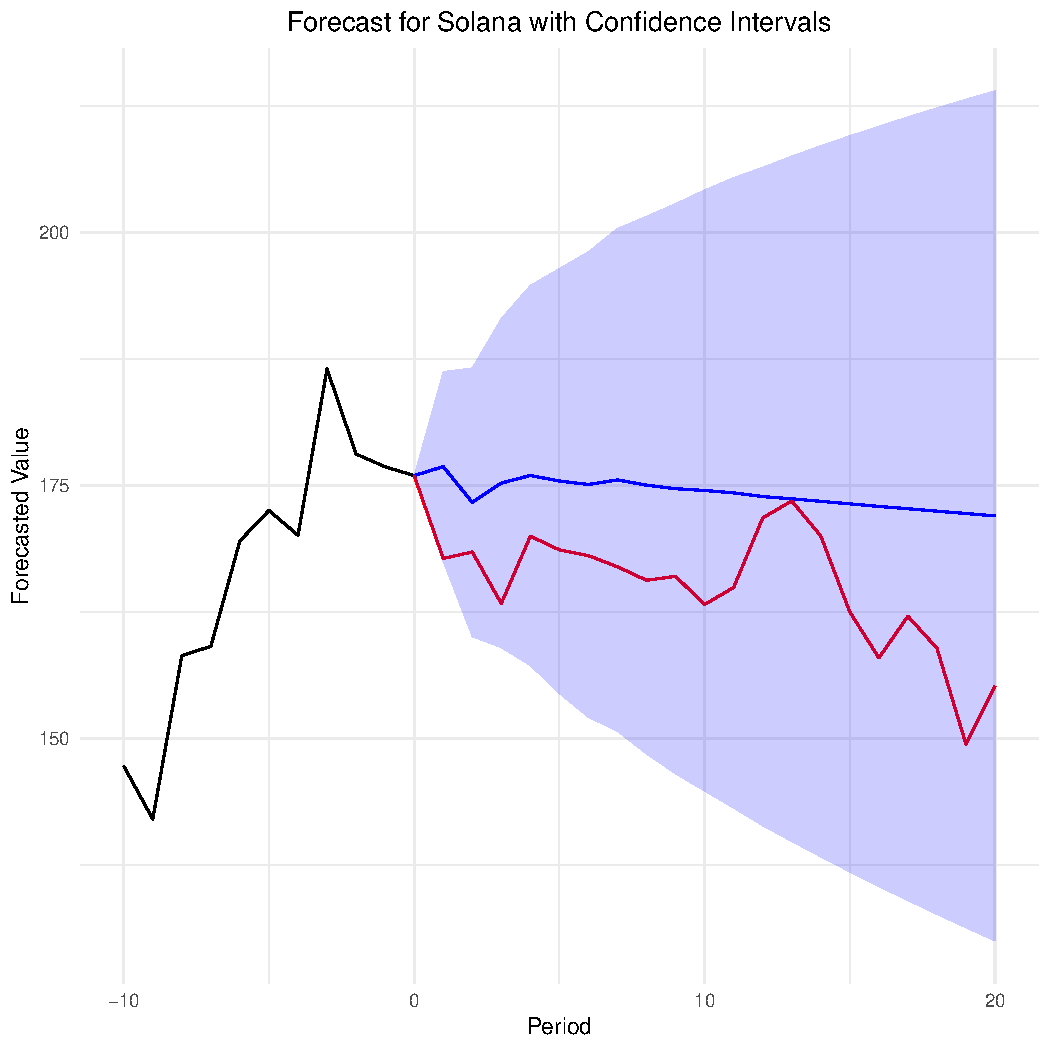
\includegraphics[width=.45\textwidth]{1.Projekt_kode/Billeder/20_day_ahed_Solana_from_Ethereum_Solana.pdf}}
  \label{}
\end{figure}

\end{comment}

\noindent For the two plots above it can be seen that on the first half of the predictions seems to be somewhat accurate for ETH and for SOL it is quite a bit off. This was to be expected, due to cryptocurrencies high volatility. Furthermore the model seem to only capture the price movement at the start of the period. ETH plot do seem to capture the direction in which the price moves, but without any nuances as the predictions seem to move in a straight line after a certain point. this is because it reverts to the long term equilibrium. It is quite positive that for both graphs the actual values lies within the $95\%$ confidence interval. Below tables with the model's level of predictability is stated:

\begin{table}[H]
\centering
\caption{Performance Metrics for Solana and Ethereum}
\begin{tabular}{lcccccc}
\toprule
\textbf{Metric} & \textbf{One-Day} & \textbf{Two-Day} & \textbf{Three-Day} & \textbf{Four-Day} & \textbf{Five-Day} \\
\midrule
\textbf{MAE} & & & & & \\
Solana        & 28.11133 & 25.22199 & 27.12728 & 27.9634 & 27.72747 \\
Ethereum      & 811.18274 & 771.61202 & 818.57316 & 845.9166 & 847.10831 \\
\midrule
\textbf{RMSE} & & & & & \\
Solana        & 31.24737 & 28.33555 & 30.14608 & 30.94042 & 30.63449 \\
Ethereum      & 953.08236 & 914.34242 & 956.88827 & 979.86588 & 979.72258 \\
\midrule
\textbf{MAPE} & & & & & \\
Solana        & 19.85790 & 17.85844 & 19.18544 & 19.77437 & 19.62114 \\
Ethereum      & 30.54404 & 29.21761 & 30.93889 & 31.95720 & 32.08274 \\
\bottomrule
\end{tabular}
\label{table:SOL_ETH_MAE_RMSE_MAPE}
\end{table}
\begin{comment}
\begin{table}[H]
\centering
\caption{Performance Metrics for Ethereum and Solana}
\begin{tabular}{lcccccc}
\toprule
\textbf{Metric} & \textbf{One-Day} & \textbf{Two-Day} & \textbf{Three-Day} & \textbf{Four-Day} & \textbf{Five-Day} \\
\midrule
\textbf{MAE} & & & & & \\
Ethereum      & 813.35 & 775.77 & 825.34 & 855.57 & 859.12 \\
Solana        & 28.06  & 25.11  & 26.96  & 27.77  & 27.52  \\
\midrule
\textbf{RMSE} & & & & & \\
Ethereum      & 955.04 & 918.29 & 963.20 & 988.58 & 990.43 \\
Solana        & 31.19  & 28.23  & 29.98  & 30.75  & 30.42  \\
\midrule
\textbf{MAPE} & & & & & \\
Ethereum      & 30.62  & 29.36  & 31.18  & 32.29  & 32.50  \\
Solana        & 19.82  & 17.78  & 19.07  & 19.64  & 19.47  \\
\bottomrule
\end{tabular}
\end{table}
From the table it stand out the prediction for Ripple in both the models in which it is represented. the two models are able to predict with an accuracy of less than $10\%$ in almost all cases.
\end{comment}

\noindent  
The MAPE is off by $19\%$ and $30\%$ for the one-day-ahead predictions respectively. Furthermore the prediction accuracy do not seem to deteriorate significantly over five days and an interesting observation is that all three mean errors for SOL are smaller for five-day-ahead compared to the one-day-ahead prediction. The relatively low MAPE for solana indicates it is somewhat descend, and therefore could be used for decision making. The ETH model is more unreliable when predicting than when predicting for SOL.
\pause

\subsection{Johansen}
Like with Engel Granger forecast, we first inspect the 20-day-ahead prediction plots. 

\begin{figure}[H]
  \centering
  \subfloat[][Bitcoin]{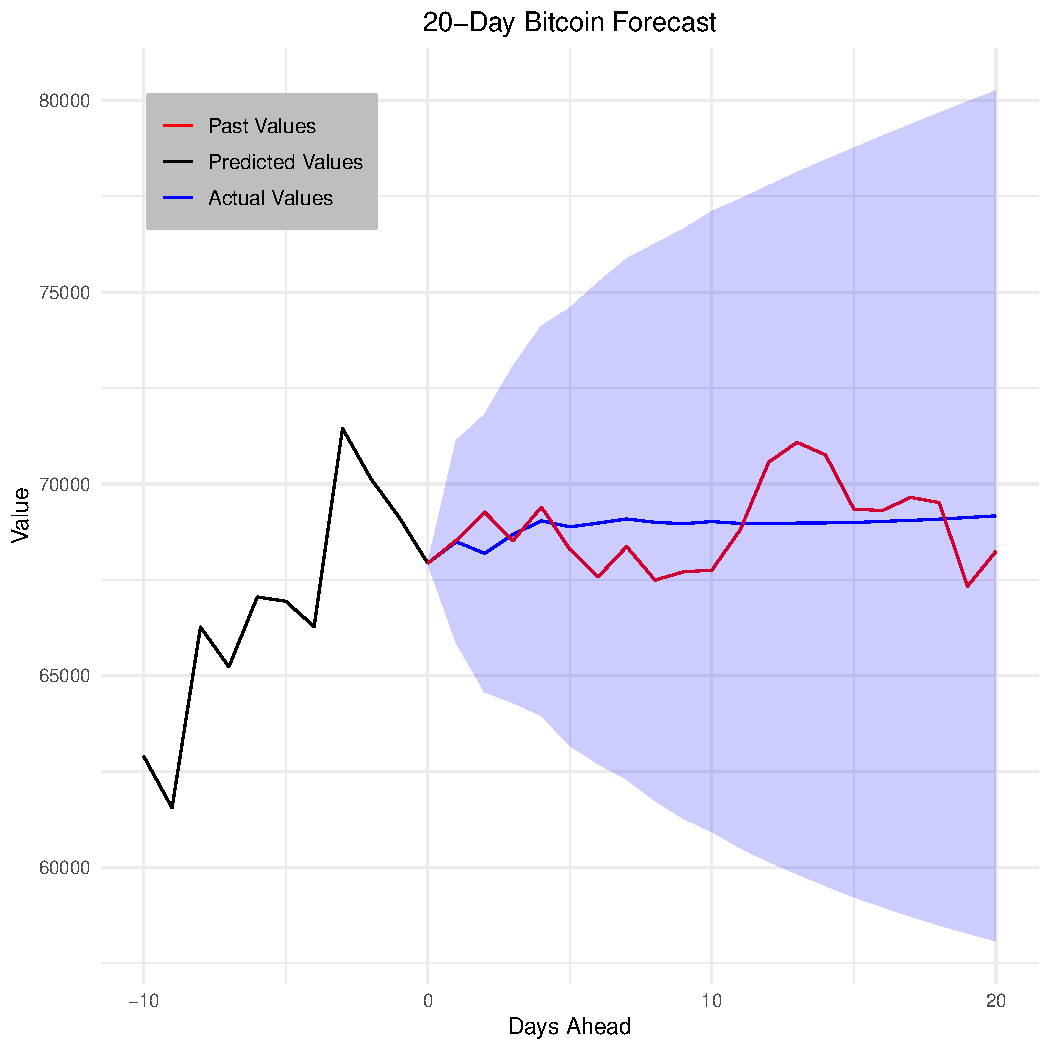
\includegraphics[width=.45\textwidth]{1.Projekt_kode/Billeder/20_day_ahead_Bitcoin_from_johanson.pdf}}\quad
  \subfloat[][Ethereum]{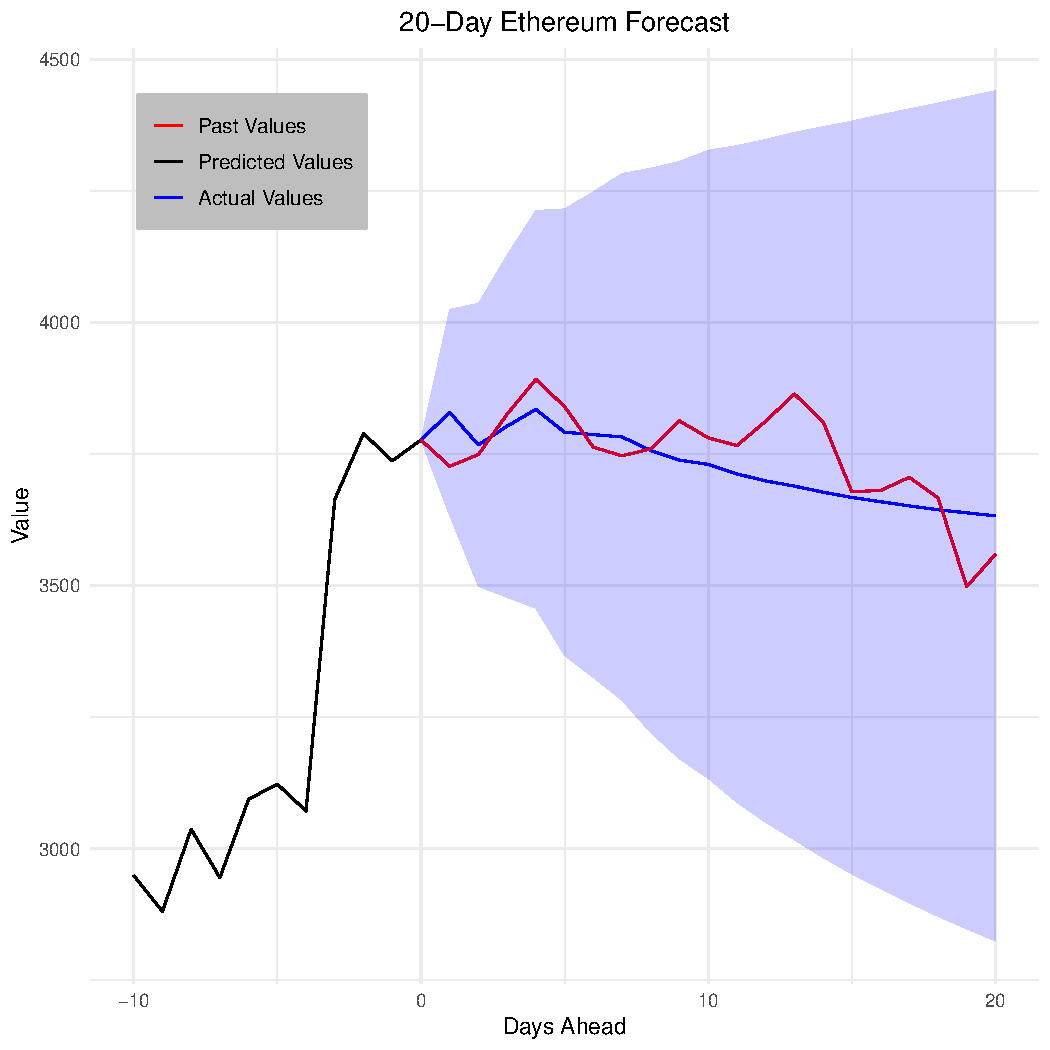
\includegraphics[width=.45\textwidth]{1.Projekt_kode/Billeder/20_day_ahead_Ethereum_from_johanson.pdf}}\\
  \subfloat[][Rippe]{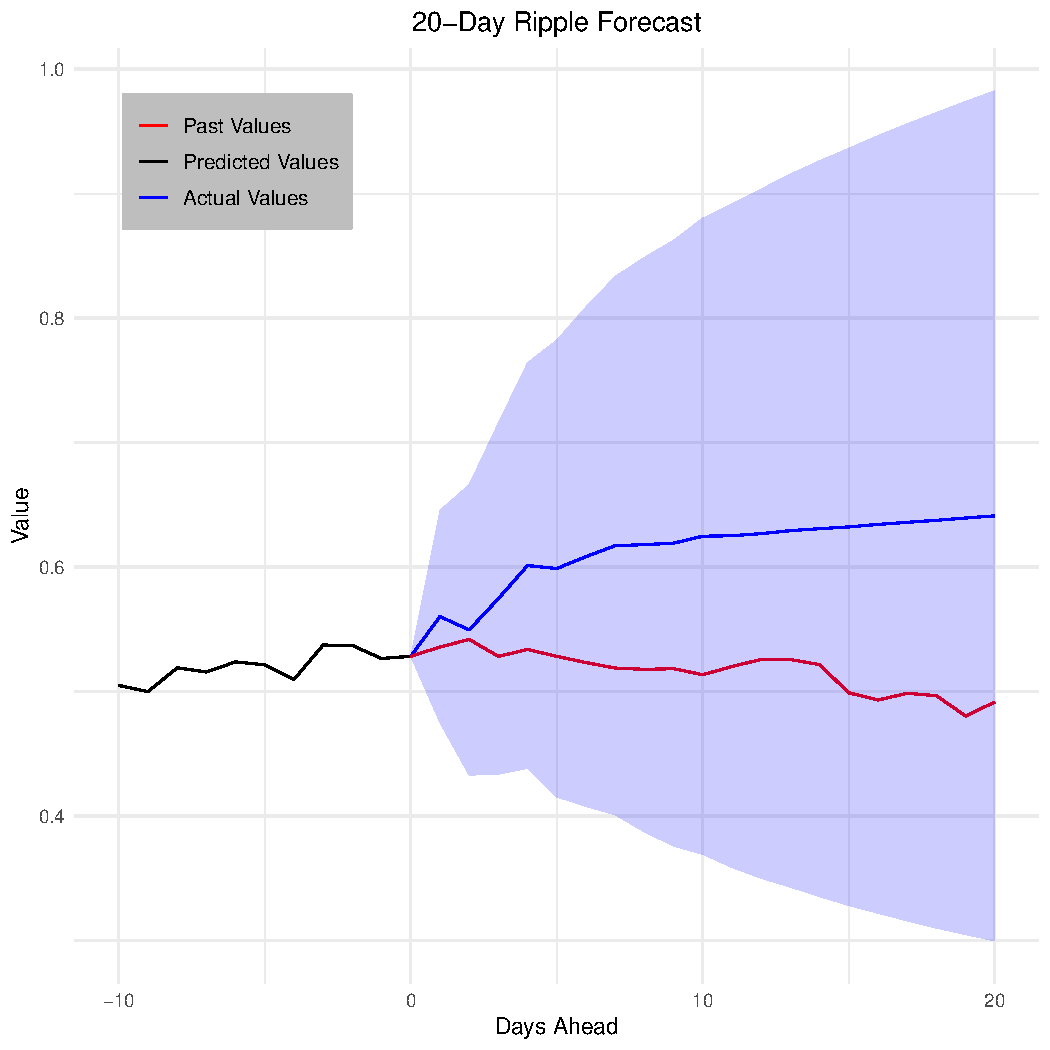
\includegraphics[width=.45\textwidth]{1.Projekt_kode/Billeder/20_day_ahead_Ripple_from_johanson.pdf}}\quad
  \subfloat[][Solana]{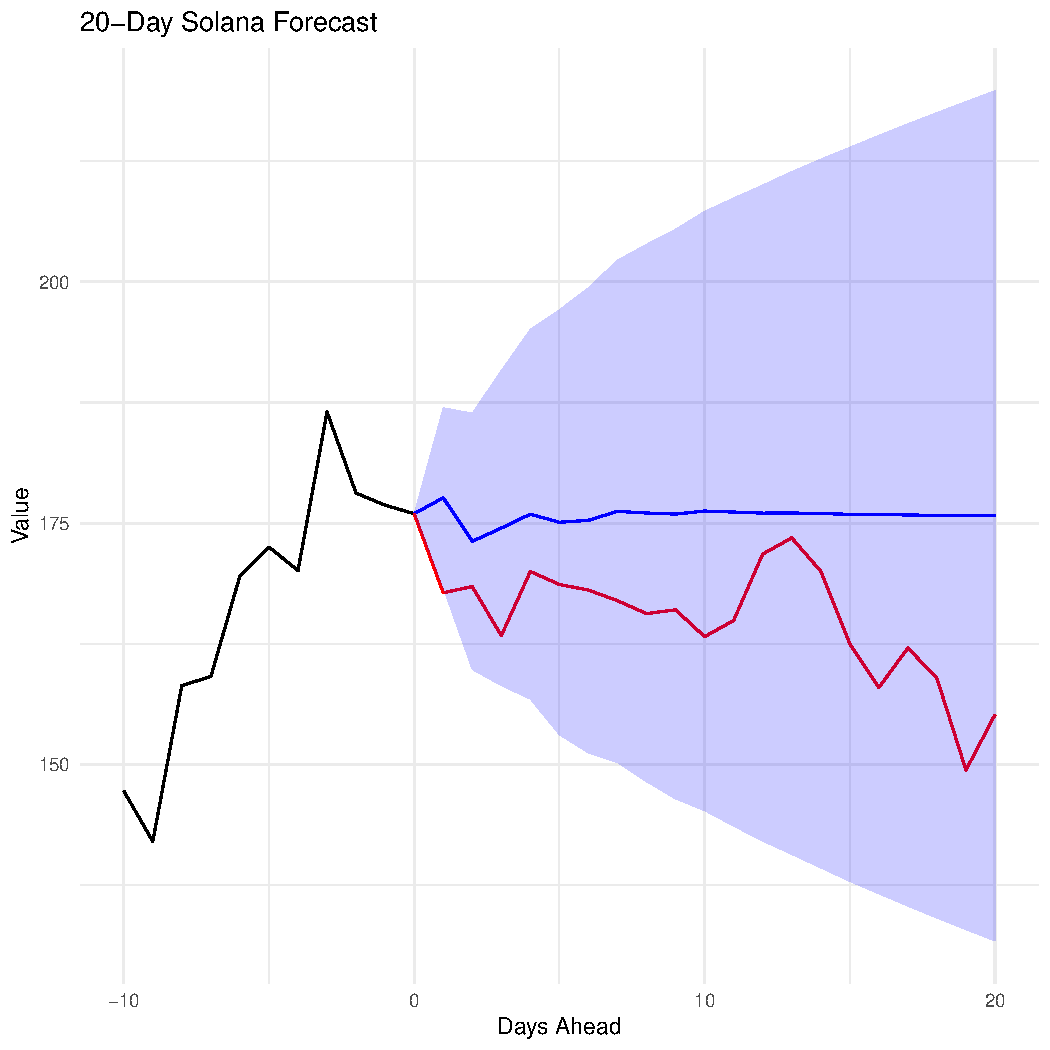
\includegraphics[width=.45\textwidth]{1.Projekt_kode/Billeder/20_day_ahead_Solana_from_johanson.pdf}}
  \caption{20-day-ahead Predictions}
  \label{fig:20_day_Johansen}
\end{figure}
\noindent The plots seems to be somewhat accurate. All the actual values lies within confidence interval. Furthermore the model captures the movement somewhat in the start. Looking at bitcoin and ethereum the first quarter of predictions looks to be quite good. For Bitcoin the first prediction is so good that the lines overlap each other. The prediction do seem to move in a straight line from a certain point.

\begin{table}[H]
\centering
\caption{Performance Metrics for Bitcoin, Ethereum, Solana, and Ripple}
\begin{tabular}{lccccc}
\toprule
\textbf{Metric} & \textbf{One-Day} & \textbf{Two-Day} & \textbf{Three-Day} & \textbf{Four-Day} & \textbf{Five-Day} \\
\midrule
\textbf{MAE} & & & & & \\
Bitcoin   & 436.5510 & 1360.4544 & 2096.0190 & 2372.9510 & 2839.9210 \\
Ethereum  &  29.4897 &   82.8389 &  112.3955 &  128.4171 &  154.1226 \\
Solana    &   5.3342 &    6.5635 &    8.9984 &   11.7554 &   10.2188 \\
Ripple    &   0.0118 &    0.0270 &    0.0461 &    0.0431 &    0.0531 \\
\midrule
\textbf{RMSE} & & & & & \\
Bitcoin   & 514.2976 & 1791.1630 & 2611.2730 & 2950.6350 & 3584.3680 \\
Ethereum  &  36.4638 &  106.7405 &  144.6352 &  162.4643 &  209.4623 \\
Solana    &   5.3489 &    8.0663 &   11.1579 &   14.3040 &   13.0975 \\
Ripple    &   0.0158 &    0.0317 &    0.0529 &    0.0506 &    0.0619 \\
\midrule
\textbf{MAPE} & & & & & \\
Bitcoin   &   0.7173 &    2.2203 &    3.4205 &    3.8782 &    4.6632 \\
Ethereum  &   0.9707 &    2.9081 &    3.9211 &    4.5413 &    5.5665 \\
Solana    &   3.6096 &    4.4267 &    6.0703 &    7.8966 &    6.8306 \\
Ripple    &   2.0972 &    5.1196 &    8.8016 &    8.0928 &   10.1982 \\
\bottomrule
\end{tabular}
\label{fig:johansen_RMSE_MAE_MAPE}
\end{table}
\noindent In the table it can be seen that the MAE gets larger, the longer into the future we predict, this is to be expected, due to the high volatility of cryptocurrencies. The MAPE especially for ond-day-ahead is quint low across the board with bitcoin standing out as the best, with an prediction error of $0.72\%$ and reaching an error at five-day-ahead prediction of $4.66\%$. Just a single prediction namely five-day-ahead for Ripple is larger than $10\%$.\\


\noindent \textbf{Comparison of Engel Granger and Johansen}\\

\noindent First looking at the plots, the predictions looks better for the Johansen model. Both Engel Granger and Johansen plots seems to behave similar, as they capture some movement at the start, and then moves in a straight line, this is expected and it is caused by the error correction.
Secondly looking the prediction errors. Here it becomes very clear that the prediction accuracy is significantly better for the model build by Johansen compared to the model build by Engel Granger. The MAPE for Johansen only have a single day-ahead prediction which is off by more than $10\%$ and most day-ahead predictions with a deviation from the true value with less than $5\%$. Compared to the Engel Granger, which do not have a single prediction which is off by less than $17\%$. This means the Johansen's worst prediction is significantly better the the Engel Granger's best prediction.\\
It is concluded that the Engel Granger model is somewhat accurate while the Johansen model is quite accurate. Furthermore, we conclude that the Johansen model is the by far the best at forecasting.